\documentclass[uplatex,dvipdfmx,ja=standard,a4paper]{bxjsarticle}
%引用:https://qiita.com/rityo_math/items/efd44bc8f9229e014237
\usepackage[hiresbb]{graphicx}
\usepackage{array}%表組を微妙に改善
\usepackage{wrapfig}%図の回り込み
\usepackage{tikz}%https://www.mathcha.io/ が便利
\usetikzlibrary{shadows}
\usepackage{otf}%フォントメトリックがまともになる
\usepackage[T1]{fontenc}%上と同様
\usepackage{lmodern}%デフォルト欧文フォントを使う時だけ、いらんかも
\usepackage{comment}%複数行コメント
\usepackage{amsmath,amssymb,amsthm}%
\usepackage{amsfonts}%おなじみの数式パッケージたち
\usepackage{mathtools}%数式コマンドを追加
\usepackage{bbm,bm}%太字ベクトル
\usepackage[hidelinks]{hyperref}%ハイパーリンクが貼れる
\usepackage{pxjahyper}%リハイパーンクを日本語に対応
\usepackage{physics}%偏微分とかが簡単に書ける
\usepackage{float}%画像とかの配置を強制できる
\usepackage{cancel}%打ち消し線が書ける
\usepackage{tcolorbox}
\tcbuselibrary{breakable, skins, theorems}%定理環境
\usepackage{xcolor}
\usepackage{listings}%日本語入りのソースコードが書ける
\usepackage{../packages/jlisting}
\usepackage{../packages/texex}%自作パッケージ2020あるいは2021 C:\texlive\2020\texmf-dist\tex\uplatex\texex

\begin{document}

\title{test}
\author{062100873 髙柳海斗}
\date{\today}
\maketitle

\begin{figure}[h]
  \centering
  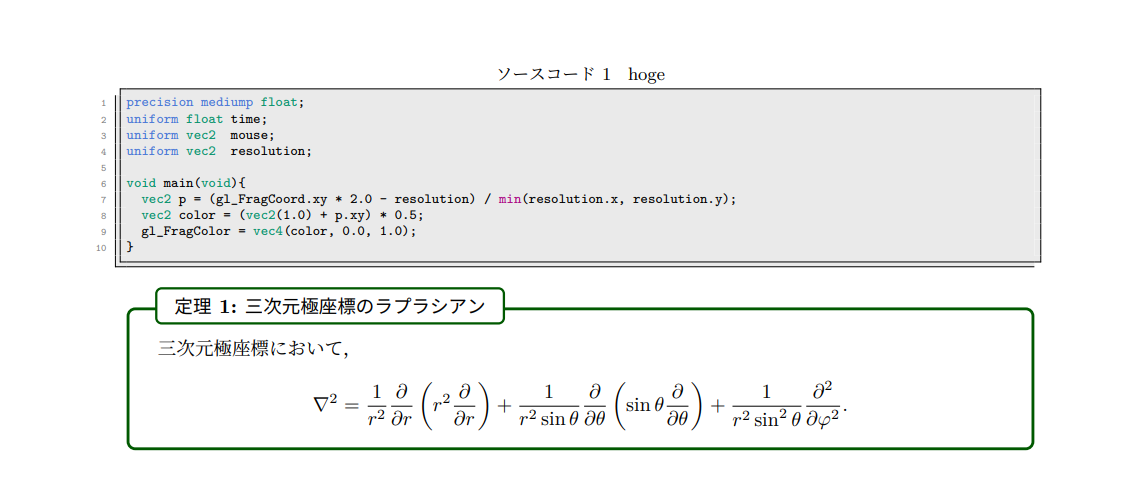
\includegraphics[keepaspectratio, width=3cm,clip]{hoge.png}
  \caption{fig1}
  \label{fig:1}
\end{figure}

\begin{table}[h]
  \centering
  \caption{table1}
  \label{table:1}
  \begin{tabular}{cll}
    \hline
    系列1 & 系列2 & 系列3 \\
    \hline
    要素 & 要素 & 要素 \\[-4pt]
    要素 & 要素 & 要素 \\[-4pt]
    要素 & 要素 & 要素 \\
    \hline
  \end{tabular}
\end{table}

\begin{figure}[h]
  \centering
  \begin{minipage}[t]{0.24\columnwidth}
    \centering
    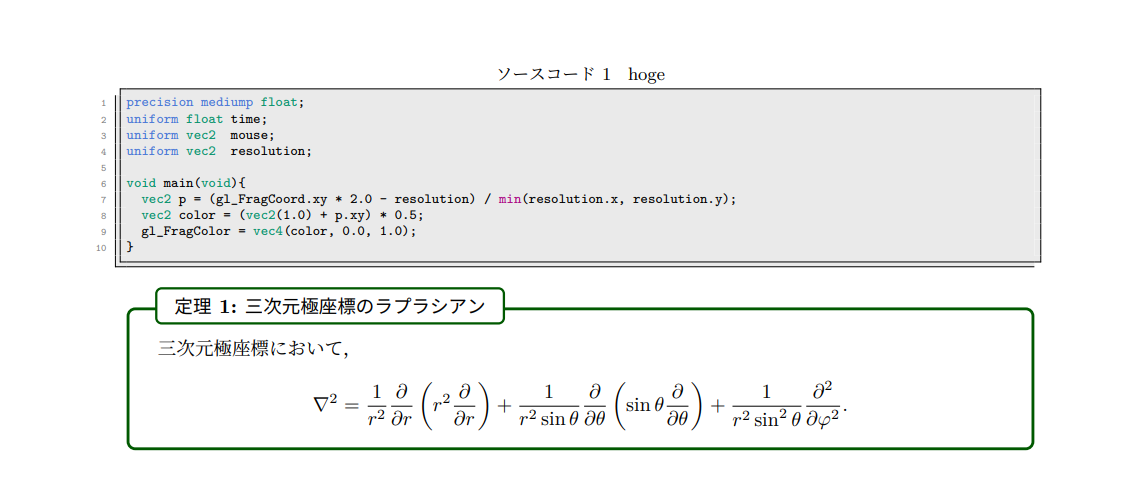
\includegraphics[keepaspectratio, width=\columnwidth,clip]{hoge.png}
    \caption{fig2}
    \label{fig:2}
  \end{minipage}
  \begin{minipage}[t]{0.24\columnwidth}
    \centering
    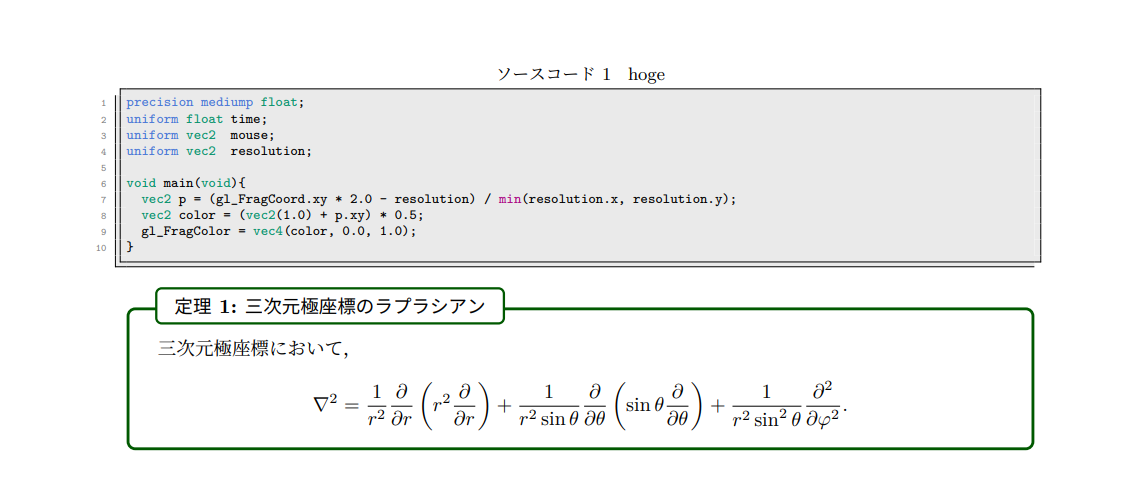
\includegraphics[keepaspectratio, width=\columnwidth,clip]{hoge.png}
    \caption{fig3}
    \label{fig:3}
  \end{minipage}
  \begin{minipage}[t]{0.24\columnwidth}
    \centering
    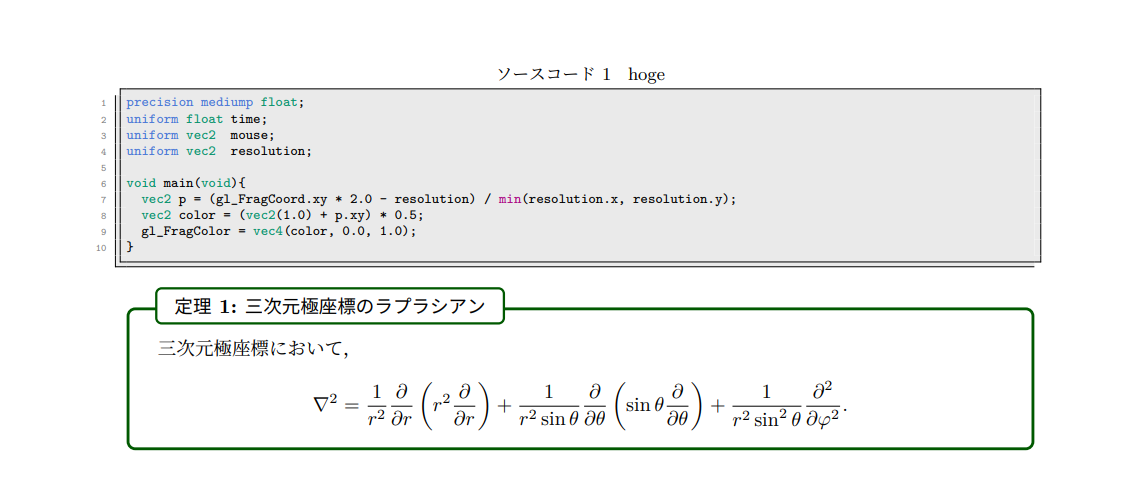
\includegraphics[keepaspectratio, width=\columnwidth,clip]{hoge.png}
    \caption{fig4}
    \label{fig:4}
  \end{minipage}
  \begin{minipage}[t]{0.24\columnwidth}
    \centering
    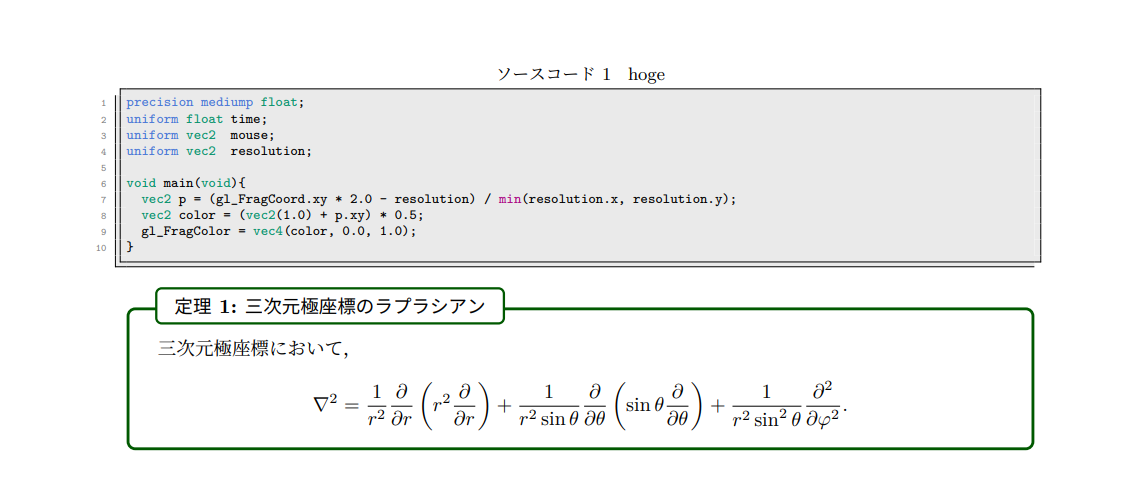
\includegraphics[keepaspectratio, width=\columnwidth,clip]{hoge.png}
    \caption{fig5}
    \label{fig:5}
  \end{minipage}
\end{figure}

\begin{wraptable}{r}{13zw}
  \vspace*{-\intextsep}
  \caption{table2}
  \label{table:2}
  \begin{tabular}{cll}
    \hline
    系列1 & 系列2 & 系列3 \\
    \hline
    要素 & 要素 & 要素 \\[-4pt]
    要素 & 要素 & 要素 \\[-4pt]
    要素 & 要素 & 要素 \\
    \hline
  \end{tabular}
\end{wraptable}
この下になんか書くほげふにふがぴよ
ああああああああああああああああああ
あああああああああああああああああああああああああ
あいうえおかきくけこあいうえおかきくけこあいうえおかきくけこ
あいうえおかきくけこあいうえおかきくけこあいうえおかきくけこ
あいうえおかきくけこあいうえおかきくけこあいうえおかきくけこ
あいうえおかきくけこあいうえおかきくけこあいうえおかきくけこ
あいうえおかきくけこあいうえおかきくけこあいうえおかきくけこ
あいうえおかきくけこあいうえおかきくけこあいうえおかきくけこ
あいうえおかきくけこあいうえおかきくけこあいうえおかきくけこ
あいうえおかきくけこあいうえおかきくけこあいうえおかきくけこ
あいうえおかきくけこあいうえおかきくけこあいうえおかきくけこ
あいうえおかきくけこあいうえおかきくけこあいうえおかきくけこ
あいうえおかきくけこあいうえおかきくけこあいうえおかきくけこ
あいうえおかきくけこあいうえおかきくけこあいうえおかきくけこ

\begin{wrapfigure}{r}{10zw}
  \vspace*{-\intextsep}
  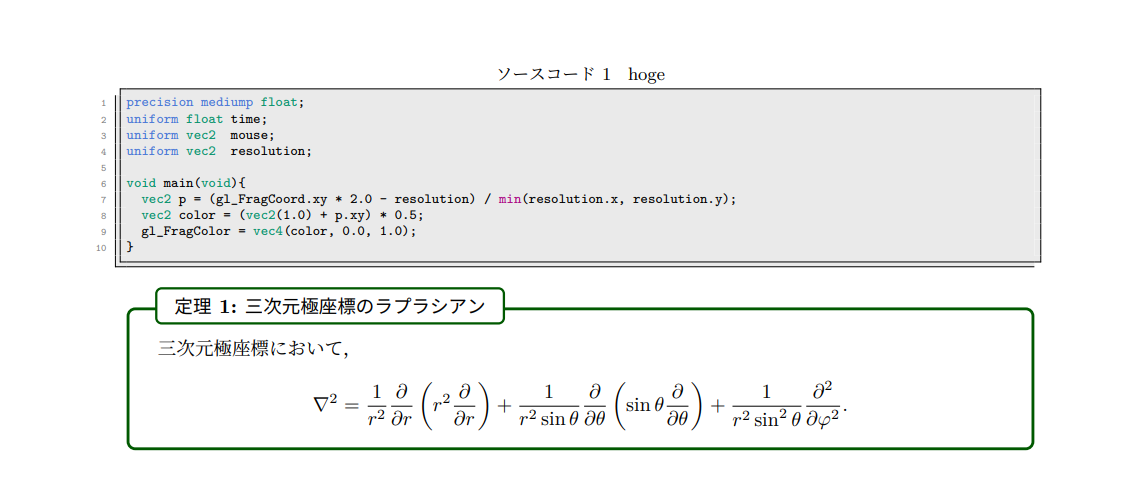
\includegraphics[keepaspectratio, width=10zw,clip]{hoge.png}
  \caption{fig6}
  \label{fig:6}
\end{wrapfigure}

この下になんか書くほげふにふがぴよ
ああああああああああああああああああ
あああああああああああああああああああああああああ
あいうえおかきくけこあいうえおかきくけこあいうえおかきくけこ
あいうえおかきくけこあいうえおかきくけこあいうえおかきくけこ
あいうえおかきくけこあいうえおかきくけこあいうえおかきくけこ
あいうえおかきくけこあいうえおかきくけこあいうえおかきくけこ
あいうえおかきくけこあいうえおかきくけこあいうえおかきくけこ
あいうえおかきくけこあいうえおかきくけこあいうえおかきくけこ
あいうえおかきくけこあいうえおかきくけこあいうえおかきくけこ
あいうえおかきくけこあいうえおかきくけこあいうえおかきくけこ
あいうえおかきくけこあいうえおかきくけこあいうえおかきくけこ
あいうえおかきくけこあいうえおかきくけこあいうえおかきくけこ
あいうえおかきくけこあいうえおかきくけこあいうえおかきくけこ
あいうえおかきくけこあいうえおかきくけこあいうえおかきくけこ
\end{document}